\documentclass[a4paper,12pt]{article}

\usepackage[utf8]{inputenc}
\usepackage[brazil]{babel}
\usepackage{graphicx}
\usepackage{geometry}
\usepackage{caption}
\usepackage{booktabs}
\usepackage{longtable}

\geometry{margin=1in}
 
\title{Modelo Relacional UML da Aplicação CAMAAR\\
\large Sistema de Avaliação de Turmas}

\author{Kelven Dias\\
Universidade de Brasília - UnB\\
Departamento de Ciência da Computação}

\date{Novembro de 2025}
 
\begin{document}
 
\maketitle

\begin{abstract}
Este documento apresenta o modelo relacional UML da aplicação CAMAAR (Sistema de Avaliação de Turmas), desenvolvida em Ruby on Rails para gerenciamento de avaliações acadêmicas. O sistema permite a gestão completa de turmas, docentes, discentes, templates de formulários, avaliações e respostas, integrando-se com dados do SIGAA.
\end{abstract}
 
\section{Introdução}

A aplicação \textbf{CAMAAR} é um sistema desenvolvido em \textit{Ruby on Rails 8.1.1}, utilizando Ruby 3.4.1, projetado para gerenciar avaliações de turmas acadêmicas na Universidade de Brasília. O sistema oferece funcionalidades para criação de templates de formulários, aplicação de avaliações, coleta e análise de respostas, além de integração com dados do SIGAA (Sistema Integrado de Gestão de Atividades Acadêmicas).

Este relatório apresenta o modelo relacional UML completo da aplicação, descrevendo suas entidades principais, atributos, relacionamentos e regras de negócio implementadas.
 
\section{Entidades Principais}

\subsection{Usuário}

Entidade base para todos os usuários do sistema, utilizando herança de tabela única (Single Table Inheritance - STI) para Docente e Dicente.

\begin{itemize}
    \item \textbf{usuario}: Identificador único do usuário (chave primária) - string
    \item \textbf{nome}: Nome completo do usuário
    \item \textbf{email}: Email institucional (único)
    \item \textbf{formacao}: Nível de formação (graduando, mestrado, doutorado)
    \item \textbf{ocupacao}: Tipo de ocupação (docente/dicente)
    \item \textbf{password\_digest}: Senha criptografada (bcrypt)
    \item \textbf{created\_at}: Data de criação do registro
    \item \textbf{updated\_at}: Data da última atualização
\end{itemize}

\textbf{Relacionamentos}: Classe pai de Docente e Dicente (relacionamento ISA).

\textbf{Regras de Negócio}:
\begin{itemize}
    \item Email deve ser único no sistema
    \item Senha deve ter no mínimo 8 caracteres
    \item Ocupação determina o perfil de acesso (administrador/participante)
\end{itemize}

\subsection{Docente}

Especialização de Usuário representando professores.

\begin{itemize}
    \item \textbf{usuario}: Chave primária e estrangeira (FK para Usuario.usuario)
    \item \textbf{departamento}: Departamento de lotação (ex: "DEPTO CIÊNCIAS DA COMPUTAÇÃO")
    \item \textbf{titulacao}: Nível de titulação (especialização, mestrado, doutorado)
\end{itemize}

\textbf{Relacionamentos}:
\begin{itemize}
    \item Um docente pode lecionar várias turmas (1:N com Turma)
    \item Um docente pode criar várias avaliações (1:N com Avaliacao)
    \item Um docente pode criar vários templates (1:N com Template)
\end{itemize}

\subsection{Dicente}

Especialização de Usuário representando alunos.

\begin{itemize}
    \item \textbf{usuario}: Chave primária e estrangeira (FK para Usuario.usuario)
    \item \textbf{matricula}: Matrícula institucional (única)
    \item \textbf{curso}: Curso de graduação (ex: "CIÊNCIA DA COMPUTAÇÃO/CIC")
\end{itemize}

\textbf{Relacionamentos}:
\begin{itemize}
    \item Um dicente pode estar matriculado em várias turmas (1:N com Matricula)
    \item Um dicente pode responder várias avaliações (1:N com Resposta)
\end{itemize}

\subsection{Materia}

Representa disciplinas oferecidas pela instituição.

\begin{itemize}
    \item \textbf{code}: Código da matéria (chave primária) - ex: "CIC0097"
    \item \textbf{name}: Nome da matéria (ex: "BANCOS DE DADOS")
    \item \textbf{created\_at}: Data de criação do registro
    \item \textbf{updated\_at}: Data da última atualização
\end{itemize}

\textbf{Relacionamentos}: Uma matéria pode ter várias turmas (1:N com Turma).

\textbf{Dados Exemplo}:
\begin{itemize}
    \item CIC0097 - BANCOS DE DADOS
    \item CIC0105 - ENGENHARIA DE SOFTWARE
    \item CIC0202 - PROGRAMAÇÃO CONCORRENTE
\end{itemize}

\subsection{Turma}

Representa uma oferta específica de uma matéria em um semestre.

\begin{itemize}
    \item \textbf{id}: Identificador único (chave primária) - int
    \item \textbf{course\_code}: Código da matéria (FK para Materia.code)
    \item \textbf{class\_code}: Código da turma (ex: "TA")
    \item \textbf{semester}: Semestre letivo (formato: "YYYY.S", ex: "2021.2")
    \item \textbf{time}: Horário de aula (ex: "35T45")
    \item \textbf{docente\_usuario}: Docente responsável (FK para Docente.usuario)
    \item \textbf{created\_at}: Data de criação do registro
    \item \textbf{updated\_at}: Data da última atualização
\end{itemize}

\textbf{Relacionamentos}:
\begin{itemize}
    \item Uma turma pertence a uma matéria (N:1 com Materia)
    \item Uma turma tem um docente responsável (N:1 com Docente)
    \item Uma turma pode ter várias matrículas (1:N com Matricula)
    \item Uma turma pode ter várias avaliações (1:N com Avaliacao)
\end{itemize}

\subsection{Matricula}

Relacionamento entre Dicente e Turma, representando a matrícula de um aluno.

\begin{itemize}
    \item \textbf{id}: Identificador único (chave primária) - int
    \item \textbf{dicente\_usuario}: Identificador do aluno (FK para Dicente.usuario)
    \item \textbf{turma\_id}: Identificador da turma (FK para Turma.id)
    \item \textbf{status}: Status da matrícula (ativo/trancado/concluído)
    \item \textbf{enrollment\_date}: Data de matrícula
    \item \textbf{final\_grade}: Nota final do aluno
    \item \textbf{created\_at}: Data de criação do registro
    \item \textbf{updated\_at}: Data da última atualização
\end{itemize}

\textbf{Relacionamentos}:
\begin{itemize}
    \item Cada matrícula vincula um dicente a uma turma
    \item Um dicente pode ter múltiplas matrículas em turmas diferentes
    \item Uma turma pode ter múltiplas matrículas
\end{itemize}

\textbf{Regras de Negócio}:
\begin{itemize}
    \item Um aluno não pode se matricular duas vezes na mesma turma
    \item Status padrão ao criar matrícula: "ativo"
    \item Nota final aceita valores de 0.0 a 10.0
\end{itemize}

\subsection{Template}

Modelos reutilizáveis de formulários de avaliação criados por docentes.

\begin{itemize}
    \item \textbf{id}: Identificador único (chave primária) - int
    \item \textbf{docente\_usuario}: Criador do template (FK para Docente.usuario)
    \item \textbf{name}: Nome do template
    \item \textbf{description}: Descrição detalhada do template
    \item \textbf{created\_at}: Data de criação do registro
    \item \textbf{updated\_at}: Data da última atualização
\end{itemize}

\textbf{Relacionamentos}:
\begin{itemize}
    \item Um template pertence a um docente (N:1 com Docente)
    \item Um template pode ser usado em várias avaliações (1:N com Avaliacao)
\end{itemize}

\textbf{Regras de Negócio}:
\begin{itemize}
    \item Templates podem conter questões dos tipos: numérica (1-5), múltipla escolha, e texto livre
    \item Questões de múltipla escolha devem ter no mínimo 2 opções
    \item Templates devem ter ao menos uma questão
    \item Nome do template deve ser único por docente e semestre
\end{itemize}

\subsection{Avaliacao}

Representa uma avaliação específica aplicada em uma turma.

\begin{itemize}
    \item \textbf{id}: Identificador único (chave primária) - int
    \item \textbf{turma\_id}: Turma avaliada (FK para Turma.id)
    \item \textbf{docente\_usuario}: Docente responsável (FK para Docente.usuario)
    \item \textbf{template\_id}: Template utilizado (FK para Template.id, opcional)
    \item \textbf{title}: Título da avaliação
    \item \textbf{description}: Descrição detalhada (text)
    \item \textbf{due\_date}: Data limite para respostas
    \item \textbf{max\_score}: Pontuação máxima (float)
    \item \textbf{status}: Status da avaliação (rascunho/publicada/fechada)
    \item \textbf{created\_at}: Data de criação do registro
    \item \textbf{updated\_at}: Data da última atualização
\end{itemize}

\textbf{Relacionamentos}:
\begin{itemize}
    \item Uma avaliação pertence a uma turma (N:1 com Turma)
    \item Uma avaliação pertence a um docente (N:1 com Docente)
    \item Uma avaliação pode ser baseada em um template (N:0..1 com Template)
    \item Uma avaliação pode ter várias questões (1:N com Questao)
    \item Uma avaliação pode ter várias respostas (1:N com Resposta)
\end{itemize}

\textbf{Regras de Negócio}:
\begin{itemize}
    \item Avaliações no estado "rascunho" não são visíveis para alunos
    \item Avaliações "publicadas" são visíveis e podem ser respondidas
    \item Avaliações "fechadas" não aceitam mais respostas
    \item Data limite deve ser posterior à data de criação
\end{itemize}

\subsection{Questao}

Representa perguntas individuais dentro de uma avaliação.

\begin{itemize}
    \item \textbf{id}: Identificador único (chave primária) - int
    \item \textbf{evaluation\_id}: Avaliação associada (FK para Avaliacao.id)
    \item \textbf{order}: Ordem da questão na avaliação (int)
    \item \textbf{question\_text}: Texto da pergunta (text)
    \item \textbf{question\_type}: Tipo de questão (dissertativa/multipla\_escolha/numerica)
    \item \textbf{points}: Pontuação da questão (float)
    \item \textbf{created\_at}: Data de criação do registro
    \item \textbf{updated\_at}: Data da última atualização
\end{itemize}

\textbf{Relacionamentos}:
\begin{itemize}
    \item Cada questão pertence a uma avaliação (N:1 com Avaliacao)
    \item Questões são ordenadas dentro de cada avaliação
\end{itemize}

\textbf{Tipos de Questão}:
\begin{itemize}
    \item \textbf{numerica}: Escala de 1 a 5
    \item \textbf{multipla\_escolha}: Opções pré-definidas (mínimo 2)
    \item \textbf{dissertativa}: Texto livre
\end{itemize}

\subsection{Resposta}

Representa as respostas dos dicentes às avaliações.

\begin{itemize}
    \item \textbf{id}: Identificador único (chave primária) - int
    \item \textbf{evaluation\_id}: Avaliação respondida (FK para Avaliacao.id)
    \item \textbf{dicente\_usuario}: Aluno que respondeu (FK para Dicente.usuario)
    \item \textbf{submission\_date}: Data de submissão
    \item \textbf{score}: Pontuação obtida (float)
    \item \textbf{feedback}: Feedback do docente (text)
    \item \textbf{status}: Status da resposta (pendente/corrigida/atrasada)
    \item \textbf{created\_at}: Data de criação do registro
    \item \textbf{updated\_at}: Data da última atualização
\end{itemize}

\textbf{Relacionamentos}:
\begin{itemize}
    \item Cada resposta pertence a uma avaliação (N:1 com Avaliacao)
    \item Cada resposta é de um dicente (N:1 com Dicente)
\end{itemize}

\textbf{Regras de Negócio}:
\begin{itemize}
    \item Um aluno pode responder cada avaliação apenas uma vez
    \item Respostas após a data limite são marcadas como "atrasada"
    \item Todas as questões obrigatórias devem ser respondidas
    \item Formulário é bloqueado após submissão bem-sucedida
\end{itemize}

\section{Relacionamentos e Cardinalidades}

\subsection{Herança (ISA)}
\begin{itemize}
    \item Usuario $\rightarrow$ Docente (1:1, disjunta, total)
    \item Usuario $\rightarrow$ Dicente (1:1, disjunta, total)
\end{itemize}

\subsection{Relacionamentos 1:N}
\begin{itemize}
    \item Materia $\rightarrow$ Turma (1:N)
    \item Docente $\rightarrow$ Turma (1:N)
    \item Docente $\rightarrow$ Template (1:N)
    \item Docente $\rightarrow$ Avaliacao (1:N)
    \item Turma $\rightarrow$ Matricula (1:N)
    \item Turma $\rightarrow$ Avaliacao (1:N)
    \item Template $\rightarrow$ Avaliacao (1:N, opcional)
    \item Avaliacao $\rightarrow$ Questao (1:N)
    \item Avaliacao $\rightarrow$ Resposta (1:N)
    \item Dicente $\rightarrow$ Matricula (1:N)
    \item Dicente $\rightarrow$ Resposta (1:N)
\end{itemize}

\section{Modelo Relacional UML}
 
O modelo relacional UML completo da aplicação \textbf{CAMAAR} é apresentado na Figura \ref{fig:uml}. O diagrama ilustra todas as entidades, atributos, chaves primárias e estrangeiras, além dos relacionamentos e suas cardinalidades.
 
\begin{figure}[h!]
    \centering
    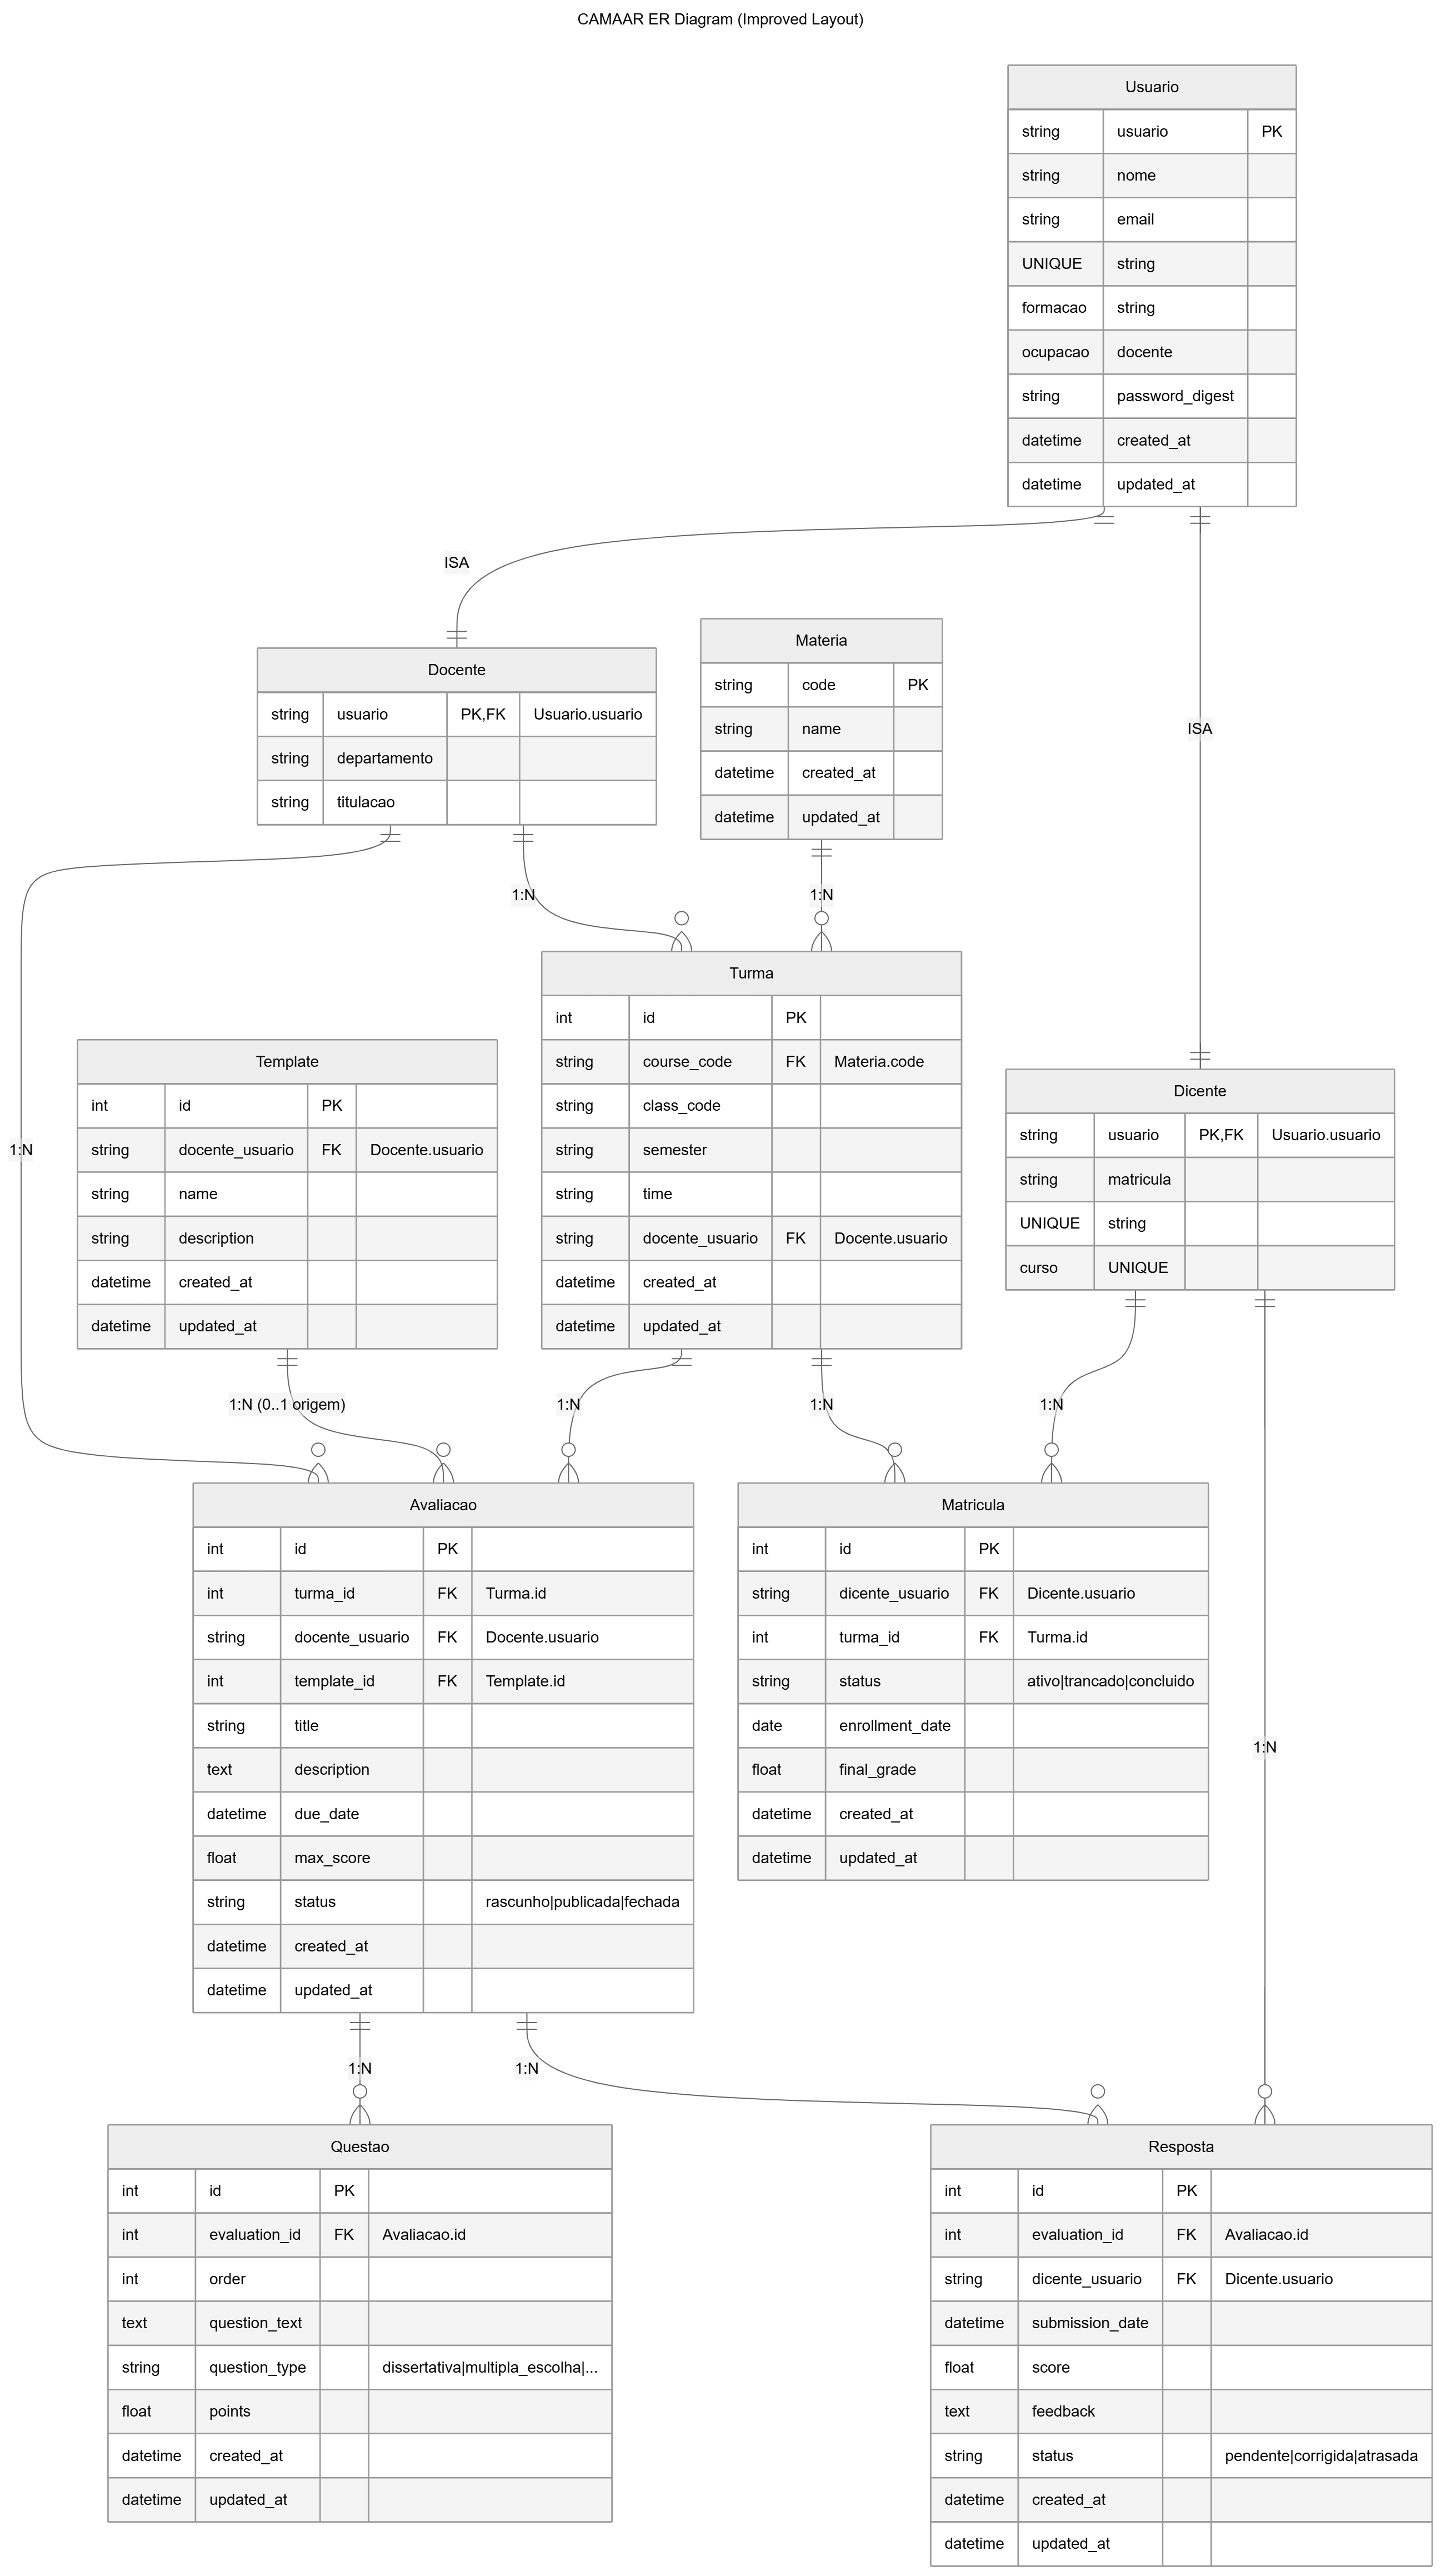
\includegraphics[width=1.0\textwidth]{CAMAAR_ER_diagram.png}
    \caption{Modelo Relacional UML da aplicação CAMAAR - Sistema de Avaliação de Turmas.}
    \label{fig:uml}
\end{figure}

\section{Considerações de Implementação}

\subsection{Tecnologias Utilizadas}
\begin{itemize}
    \item \textbf{Ruby on Rails 8.1.1}: Framework web MVC
    \item \textbf{Ruby 3.4.1}: Linguagem de programação
    \item \textbf{SQLite3}: Banco de dados (desenvolvimento/teste)
    \item \textbf{Cucumber + Capybara}: Framework BDD para testes
    \item \textbf{GitHub Actions}: CI/CD
\end{itemize}

\subsection{Padrões Adotados}

\textbf{Single Table Inheritance (STI)}: Utilizado para as entidades Usuario, Docente e Dicente, permitindo polimorfismo e reutilização de código.

\textbf{Soft Deletes}: Registros não são deletados fisicamente, apenas marcados como inativos através do campo \texttt{status}.

\textbf{Timestamps}: Todos os modelos incluem \texttt{created\_at} e \texttt{updated\_at} para auditoria.

\textbf{Validações}: Implementadas no nível de aplicação (ActiveRecord) e banco de dados (constraints).

\subsection{Segurança}
\begin{itemize}
    \item Senhas armazenadas com bcrypt (has\_secure\_password)
    \item Autenticação baseada em sessões
    \item Controle de acesso por perfil (Admin/Participante)
    \item Validação de permissões em todas as operações sensíveis
\end{itemize}

\subsection{Integração com SIGAA}

O sistema importa dados do SIGAA através de arquivos JSON:
\begin{itemize}
    \item \texttt{class\_members.json}: Dados de turmas, docentes e dicentes
    \item \texttt{classes.json}: Informações de disciplinas e ofertas
\end{itemize}

A importação evita duplicação através de validações de unicidade em campos-chave (usuario, matricula, email).

\section{Casos de Uso Principais}

\subsection{UC01: Responder Formulário (\#99)}
\textbf{Ator}: Dicente\\
\textbf{Fluxo}:
\begin{enumerate}
    \item Dicente visualiza formulários disponíveis para sua turma
    \item Sistema valida permissões de acesso
    \item Dicente preenche questões obrigatórias
    \item Sistema valida completude das respostas
    \item Sistema registra resposta e bloqueia formulário
\end{enumerate}

\subsection{UC02: Cadastrar Usuários do Sistema (\#100)}
\textbf{Ator}: Administrador\\
\textbf{Fluxo}:
\begin{enumerate}
    \item Administrador acessa módulo de cadastro de usuários
    \item Sistema solicita dados: nome, email, tipo (docente/dicente)
    \item Administrador preenche informações do usuário
    \item Sistema valida unicidade de email e matrícula
    \item Sistema cria usuário e envia email de ativação
\end{enumerate}

\subsection{UC03: Sistema de Login (\#104)}
\textbf{Ator}: Usuário (Docente/Dicente)\\
\textbf{Fluxo}:
\begin{enumerate}
    \item Usuário acessa página de login
    \item Sistema solicita credenciais (email/usuário e senha)
    \item Usuário fornece credenciais
    \item Sistema valida autenticação
    \item Sistema redireciona para dashboard apropriado ao perfil
\end{enumerate}

\subsection{UC04: Sistema de Definição de Senha (\#105)}
\textbf{Ator}: Usuário (primeiro acesso)\\
\textbf{Fluxo}:
\begin{enumerate}
    \item Usuário acessa sistema pela primeira vez
    \item Sistema detecta ausência de senha definida
    \item Sistema solicita criação de senha forte
    \item Usuário define senha (mínimo 8 caracteres)
    \item Sistema valida força da senha e confirma cadastro
\end{enumerate}

\subsection{UC05: Criar Template de Formulário (\#102)}
\textbf{Ator}: Docente\\
\textbf{Fluxo}:
\begin{enumerate}
    \item Docente acessa página de gerenciamento de templates
    \item Docente define nome e descrição
    \item Docente adiciona questões (numéricas, múltipla escolha, texto)
    \item Sistema valida regras de negócio
    \item Template é salvo e disponibilizado para criação de avaliações
\end{enumerate}

\subsection{UC06: Criar Formulário de Avaliação (\#103)}
\textbf{Ator}: Docente\\
\textbf{Fluxo}:
\begin{enumerate}
    \item Docente seleciona turma e template (opcional)
    \item Docente define título, descrição e prazo
    \item Docente configura questões e pontuação
    \item Sistema valida dados e cria avaliação em estado "rascunho"
    \item Docente publica avaliação tornando-a visível para alunos
\end{enumerate}

\subsection{UC07: Visualizar Formulários Pendentes (\#109)}
\textbf{Ator}: Dicente\\
\textbf{Fluxo}:
\begin{enumerate}
    \item Dicente acessa dashboard de formulários
    \item Sistema lista avaliações disponíveis para suas turmas
    \item Sistema destaca prazos próximos e formulários atrasados
    \item Dicente pode filtrar por turma ou status
    \item Dicente seleciona formulário para responder
\end{enumerate}

\subsection{UC08: Visualizar Resultados dos Formulários (\#110)}
\textbf{Ator}: Docente\\
\textbf{Fluxo}:
\begin{enumerate}
    \item Docente acessa página de resultados
    \item Sistema lista avaliações com respostas
    \item Docente seleciona avaliação específica
    \item Sistema exibe estatísticas consolidadas e gráficos
    \item Docente pode exportar relatório
\end{enumerate}

\subsection{UC09: Visualizar Templates Criados (\#111)}
\textbf{Ator}: Docente\\
\textbf{Fluxo}:
\begin{enumerate}
    \item Docente acessa biblioteca de templates
    \item Sistema lista templates criados pelo docente
    \item Docente pode buscar por nome ou filtrar por semestre
    \item Sistema exibe preview do template selecionado
    \item Docente pode editar, duplicar ou excluir template
\end{enumerate}

\subsection{UC10: Edição e Deleção de Templates (\#112)}
\textbf{Ator}: Docente\\
\textbf{Fluxo}:
\begin{enumerate}
    \item Docente seleciona template para editar/excluir
    \item Sistema verifica se template está em uso
    \item Para edição: docente modifica questões e salva alterações
    \item Para exclusão: sistema alerta sobre avaliações vinculadas
    \item Sistema confirma operação e atualiza registro
\end{enumerate}

\subsection{UC11: Importar Dados do SIGAA (\#98, \#108)}
\textbf{Ator}: Administrador\\
\textbf{Fluxo}:
\begin{enumerate}
    \item Administrador acessa página de importação
    \item Sistema solicita arquivos JSON
    \item Administrador seleciona arquivos
    \item Sistema valida formato e integridade
    \item Sistema importa dados evitando duplicatas
    \item Sistema exibe relatório de importação
\end{enumerate}

\subsection{UC12: Gerar Relatório do Administrador (\#101)}
\textbf{Ator}: Administrador\\
\textbf{Fluxo}:
\begin{enumerate}
    \item Administrador acessa módulo de relatórios
    \item Sistema oferece opções de filtros (período, turma, docente)
    \item Administrador seleciona parâmetros desejados
    \item Sistema processa dados e gera visualizações
    \item Administrador pode exportar em PDF, Excel ou CSV
\end{enumerate}

\section{Métricas do Projeto}

\subsection{Sprint 1 - Velocity}
\begin{longtable}{|l|p{6cm}|c|}
\hline
\textbf{ID} & \textbf{Funcionalidade} & \textbf{Pontos} \\
\hline
\endfirsthead
\hline
\textbf{ID} & \textbf{Funcionalidade} & \textbf{Pontos} \\
\hline
\endhead
\#98 & Importar dados do SIGAA (base) & 5 \\
\#99 & Responder formulário & 5 \\
\#100 & Cadastrar usuários do sistema & 3 \\
\#101 & Gerar relatório do administrador & 5 \\
\#102 & Criar template de formulário & 8 \\
\#103 & Criar formulário de avaliação & 5 \\
\#104 & Sistema de Login & 5 \\
\#105 & Sistema de definição de senha & 3 \\
\#108 & Atualizar base de dados com dados do SIGAA & 5 \\
\#109 & Visualização de formulários para responder & 3 \\
\#110 & Visualização de resultados dos formulários & 8 \\
\#111 & Visualização dos templates criados & 2 \\
\#112 & Edição e deleção de templates & 5 \\
\hline
\multicolumn{2}{|r|}{\textbf{Total (Velocity):}} & \textbf{61} \\
\hline
\end{longtable}

\subsection{Funcionalidades Bônus (Não Incluídas no Velocity)}
\begin{itemize}
    \item \textbf{\#106} - Sistema de gerenciamento por departamento (8 pontos)
    \item \textbf{\#107} - Redefinição de senha (3 pontos)
    \item \textbf{\#113} - Criação de formulário para docentes ou dicentes (5 pontos)
\end{itemize}

\section{Considerações Finais}

O modelo apresentado reflete uma arquitetura robusta e escalável para o sistema \textbf{CAMAAR}. A estrutura permite:

\begin{itemize}
    \item \textbf{Flexibilidade}: Templates reutilizáveis e tipos variados de questões
    \item \textbf{Escalabilidade}: Suporte a múltiplas turmas, matérias e semestres
    \item \textbf{Auditoria}: Timestamps e status em todas as entidades críticas
    \item \textbf{Integridade}: Relacionamentos bem definidos com constraints
    \item \textbf{Extensibilidade}: Estrutura preparada para novas funcionalidades
\end{itemize}

O sistema está em conformidade com as práticas recomendadas de desenvolvimento Rails e segue princípios SOLID, facilitando manutenção e evolução contínua.

\section*{Referências}

\begin{itemize}
    \item Ruby on Rails Guides: \texttt{https://guides.rubyonrails.org/}
    \item Cucumber Documentation: \texttt{https://cucumber.io/docs/}
    \item GitHub Repository: \texttt{https://github.com/EngSwCIC/CAMAAR}
    \item Figma Mockups: \texttt{https://www.figma.com/design/5GVzfaJSBbcXmGvuvAi7WF/}
\end{itemize}

\end{document}
